%!TEX program = lualatex
% Arquivo: Template_Estat_Texto.tex

\documentclass[a4paper,12pt]{article}

% =========================================================
% Idioma e tipografia (LuaLaTeX)
% =========================================================
\usepackage[portuguese]{babel}
\usepackage{fontspec}
\setmainfont{Latin Modern Roman}

% =========================================================
% Layout
% =========================================================
\usepackage[top=3cm,bottom=2.5cm,left=3cm,right=2.5cm]{geometry}
\usepackage{setspace}
\onehalfspacing
\usepackage{indentfirst}
\setlength{\parindent}{1.25cm}

% =========================================================
% Matemática (align*, etc.)
% =========================================================
\usepackage{amsmath}
\usepackage{amssymb}

% =========================================================
% Tabelas, listas, figuras
% =========================================================
\usepackage{booktabs}
\usepackage{array}
\usepackage{enumitem}
\setlist[itemize]{noitemsep,topsep=3pt}
\setlist[enumerate]{noitemsep,topsep=3pt}

\usepackage{graphicx}
\usepackage{float}
\usepackage{pdflscape}
\graphicspath{{./}{./imagens/}{./figuras/}}

% =========================================================
% Links
% =========================================================
\usepackage{hyperref}
\usepackage{xurl}
\hypersetup{
  colorlinks=true,
  linkcolor=black,
  urlcolor=blue,
  citecolor=black,
  pdfauthor={},
  pdftitle={}
}
\usepackage{siunitx}

\sisetup{
  output-decimal-marker = {,}
}

% =========================================================
% Dados da capa
% =========================================================
\newcommand{\Instituicao}{Universidade do Estado do Rio de Janeiro}
\newcommand{\Curso}{Física VI -- Oceanografia}
\newcommand{\Professor}{Professor: Alexandre Magno}
\newcommand{\Aluno}{Aluno: Israel Oliveira Carneiro\\ Miguel Gayani\\ José Mauro Elsas}
\newcommand{\Cidade}{Rio de Janeiro}
\newcommand{\Ano}{2026}

\title{\textbf{Título do Documento}}
\author{\Aluno}
\date{\Cidade --- \Ano}

\begin{document}

% =========================================================
% Capa (página de rosto)
% =========================================================
\begin{titlepage}
\centering
{\large \Instituicao \par}
\vspace{0.5cm}
{\large \Curso \par}
\vspace{1.0cm}

{\LARGE \textbf{Experimento 2} \par}
\vspace{0.6cm}
{\Large Lei de Ohm \par}

\begin{figure}[H]
  \centering
  
\includegraphics[width=.3\linewidth]{./uerj.jpg}
\end{figure}

\vfill



\begin{flushright}
\Aluno\\
\Professor
\end{flushright}

\vspace{1.0cm}
{\Cidade --- \Ano \par}
\end{titlepage}


\section{Objetivo}

O objetivo da prática construir o gráfico voltagem vs. corrente (utilizando valores médios) para cada e obter o valor da resistência a partir do gráfico

\section{Introdução}

O estudo da eletricidade desenvolveu-se de forma significativa entre o final do século XVIII e o início do século XIX, especialmente após a criação da pilha elétrica por Alessandro Volta, em 1800. A disponibilidade de uma fonte relativamente contínua de corrente elétrica permitiu a realização de experimentos mais sistemáticos sobre o comportamento dos circuitos e dos materiais condutores.

Nesse contexto, o físico e matemático alemão Georg Simon Ohm (1789--1854) investigou experimentalmente a relação entre a diferença de potencial aplicada a um condutor e a corrente elétrica que o atravessa. Os resultados de seus estudos foram publicados em 1827, na obra \textit{Die galvanische Kette, mathematisch bearbeitet}, cujo título pode ser traduzido como ``O circuito galvânico tratado matematicamente''. Embora suas conclusões tenham enfrentado resistência inicial por parte da comunidade científica, os trabalhos de Ohm tornaram-se fundamentais para o desenvolvimento da teoria dos circuitos elétricos.

A Primeira Lei de Ohm estabelece que, para determinados materiais e sob condições físicas constantes, especialmente de temperatura, a corrente elétrica que atravessa um condutor é diretamente proporcional à diferença de potencial aplicada entre suas extremidades. Essa relação pode ser representada por

\begin{equation}
V = R I,
\label{eq:primeira_lei_ohm}
\end{equation}

em que (V) representa a diferença de potencial elétrico, medida em volts (\si{\volt}); (I) representa a intensidade da corrente elétrica, medida em amperes (\si{\ampere}); e (R) corresponde à resistência elétrica do condutor, medida em ohms (\si{\ohm}).

Para um condutor que obedece à Primeira Lei de Ohm, denominado condutor ôhmico, a resistência elétrica permanece aproximadamente constante. Dessa forma, o gráfico da diferença de potencial em função da corrente elétrica apresenta comportamento linear, e o coeficiente angular da reta corresponde ao valor da resistência do componente. Entretanto, materiais ou dispositivos que não apresentam essa proporcionalidade são classificados como não ôhmicos.

A verificação experimental da Primeira Lei de Ohm permite analisar o comportamento elétrico de um resistor, determinar sua resistência a partir de medidas de tensão e corrente e comparar o valor experimental com o valor nominal indicado pelo fabricante. Além disso, o experimento contribui para a compreensão do funcionamento de circuitos elétricos e das limitações associadas às medições realizadas em laboratório.

\section{Materiais utilizados}

Foram os seguintes os materiais utilizados para a execução do Experimento.

\begin{enumerate}[label=\alph*.]
    \item Voltímetro analógico com pontas de prova. \par\vspace{0.5\baselineskip}

    \item Miliamperímetro analógico \par\vspace{0.5\baselineskip}

    \item Fonte de alimentação. \par\vspace{0.5\baselineskip}
    
    \item Resistor de $\SI{390}{\,\ohm}\,\pm 5\%$. \par\vspace{0.5\baselineskip}
    
    \item Multímetro digital. \par\vspace{0.5\baselineskip}
    
    \item Eletrodos em placas. \par\vspace{0.5\baselineskip}
  
    \end{enumerate}

\section{Metodologia}

    Na montagem da bandeja com eletrodos, eletrólito e papel milimetrado sob o fundo transparente da bandeja, pode-se definir a linha mais espessa entre as hastes dos eletrodos como o zero da escala no eixo y e a distância entre os eletrodos é de 10cm. Assim, a ponta de prova positiva deve ser mergulhada verticalmente em (1,0). Então fizemos as medidas em x variando em $y = (0, 1, 3, 5, -1, -3, -5)$.

    As medições das linhas equipontenciais foram registradas em 5 tabelas diferentes.

\section{Medições}

    \begin{table}[H]
    \centering
        \caption{Tensão: \SI{1,21}{V}}
        \begin{tabular}{cc}
            \toprule
            \shortstack{Posição em $x$} & \shortstack{Posição em y}\\
            \midrule
            1,0   & 0\\
            1,0   & 1\\
            0,8   & 3\\
            0,7   & 5\\
            0,9   & -1\\
            0,8   & -3\\
            0,5   & -5\\
            \bottomrule
        \end{tabular}
       
        \label{tab:1,21V}
\end{table}

    \begin{table}[H]
    \centering
        \caption{Tensão: \SI{2,83}{V
        }}
        \begin{tabular}{cc}
            \toprule
            \shortstack{Posição em $x$} & \shortstack{Posição em y}\\
            \midrule
            3,0   & 0\\
            3,1   & 1\\
            3,1   & 3\\
            2,7   & 5\\
            2,7   & -1\\
            2,5   & -3\\
            2,3   & -5\\
            \bottomrule
        \end{tabular}
               \label{tab:2,83V}
    \end{table}

        \begin{table}[H]
    \centering
        \caption{Tensão: 4,4V}
        \begin{tabular}{cc}
            \toprule
            \shortstack{Posição em $x$} & \shortstack{Posição em y}\\
            \midrule
            5,0   & 0\\
            5,0   & 1\\
            4,4   & 3\\
            4,7   & 5\\
            5,0   & -1\\
            4,8   & -3\\
            4,7   & -5\\
            \bottomrule
        \end{tabular}
               \label{tab:4,4V}
    \end{table}

            \begin{table}[H]
    \centering
        \caption{Tensão: 5,92V}
        \begin{tabular}{cc}
            \toprule
            \shortstack{Posição em $x$} & \shortstack{Posição em y}\\
            \midrule
            7,0   & 0\\
            7,0   & 1\\
            6,9   & 3\\
            6,8   & 5\\
            6,9   & -1\\
            6,9   & -3\\
            7,0   & -5\\
            \bottomrule
        \end{tabular}
               \label{tab:5,92V}
    \end{table}

                \begin{table}[H]
    \centering
        \caption{Tensão: 7,5V}
        \begin{tabular}{cc}
            \toprule
            \shortstack{Posição em $x$} & \shortstack{Posição em y}\\
            \midrule
            9,0   & 0\\
            8,8   & 1\\
            9,0   & 3\\
            9,0   & 5\\
            8,9   & -1\\
            8,7   & -3\\
            9,0   & -5\\
            \bottomrule
        \end{tabular}
               \label{tab:7,5V}
    \end{table}

\section{resultados}

Diferenças em relação à primeira leitura:

\begin{enumerate}[label=\alph*.]
    \item $\Delta_1 =  2,83 - 1,21 = 1,62$
    \item $\Delta_2 =  4,40 - 1,21 = 3,19$
    \item $\Delta_3 =  5,92 - 1,21 = 4,71$
    \item $\Delta_4 =  7,50 - 1,21 = 6,21$
\end{enumerate}

\section{Gráfico}

Ver anexo.

\newpage

\begin{figure}[H]
    \centering
    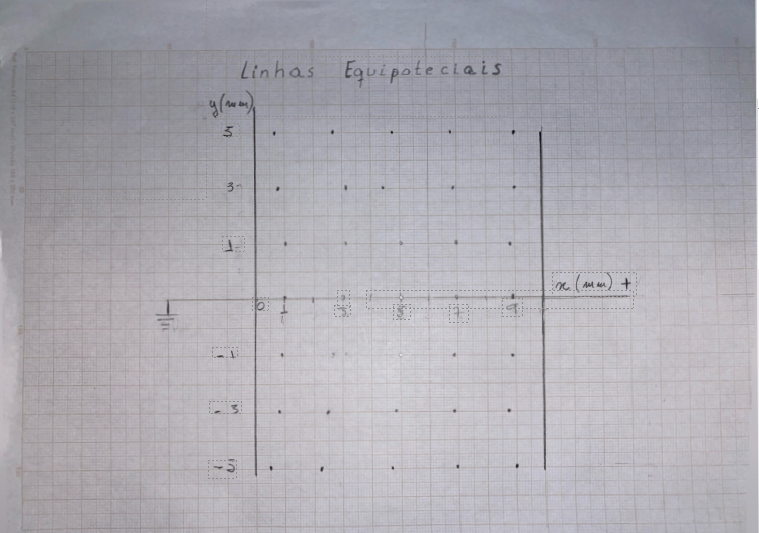
\includegraphics[angle= 90,
    origin=c,
    height=0.8\textheight]
    {./Figs/linhas_equipontenciais.png}
    \caption{linhas Equipotenciais.}
    \label{graf:linhas}
\end{figure}

\end{document}